\documentclass{standalone}

\usepackage{tikz}

\usetikzlibrary{calc,decorations.markings}

% TikZ Styles for different node types
\tikzset{
  anchornode/.style={
    forestgreen,
    minimum width=0pt
  },
  treeline/.style={
    forestgreen
  },
  starline/.style={
    staryellow
  },
  linepot/.style={
    treepot
  },
  lineball/.style={
    baublered
  },
}

% custom colours
\usepackage{xcolor}

\definecolor{forestgreen}{HTML}{3E8D3E}
\definecolor{treepot}{HTML}{5e2f0d}
\definecolor{staryellow}{HTML}{ffd500}
\definecolor{baublered}{HTML}{c60000}

% counters (useful for indexing and as helper variables)
\newcounter{id}
\newcounter{id2}
\newcounter{id3}

\begin{document}

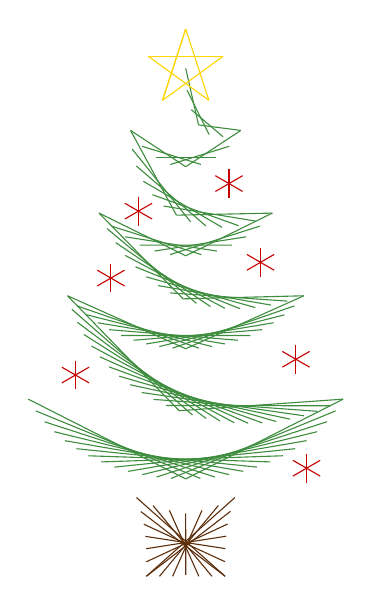
\begin{tikzpicture}[every node/.style={inner sep=0pt,outer sep=0pt}] 
  % draw all nodes 
  \foreach \x in {0.0,0.03846153846,...,1.0} {
    \path (-2,0) to[out=-60,in=240] 
      node[anchornode,pos=\x] (\the\value{id}){} (2,0) ; 
    \stepcounter{id}
  }
  \foreach \x in {0.0,0.04166666667,...,1.0} {
    \path (2,0) to[out=210,in=-75] 
      node[anchornode,pos=\x] (\the\value{id}){} (-3/4*2,5.25-3/4*5.25);  
    \stepcounter{id}
  }
  \foreach \x in {0.0,0.05,...,1.0} {
    \path (-3/4*2,5.25-3/4*5.25) to[out=-50,in=230] 
      node[anchornode,pos=\x] (\the\value{id}){} (3/4*2,5.25-3/4*5.25);  
    \stepcounter{id}
  }
  \foreach \x in {0.0,0.0625,...,1.0} {
    \path (3/4*2,5.25-3/4*5.25) to[out=200,in=-65,looseness=1.1] 
      node[anchornode,pos=\x] (\the\value{id}){} (-2.2/4*2,5.25-2.2/4*5.25);  
    \stepcounter{id}
  }
  \foreach \x in {0.083333333,0.166666666,...,1.0} {
    \path (-2.2/4*2,5.25-2.2/4*5.25) to[out=-50,in=230,looseness=1.1] 
      node[anchornode,pos=\x] (\the\value{id}){} (2.2/4*2,5.25-2.2/4*5.25);  
    \stepcounter{id}
  }
  \foreach \x in {0,0.083333333,0.166666666,...,1.0} {
    \path (2.2/4*2,5.25-2.2/4*5.25) to[out=210,in=-90,looseness=1.2] 
      node[anchornode,pos=\x] (\the\value{id}){} (-1.4/4*2,5.25-1.4/4*5.25);  
    \stepcounter{id}
  }
  \foreach \x in {0.0,0.125,...,1.0} {
    \path (-1.4/4*2,5.25-1.4/4*5.25) to[out=-60,in=240,looseness=1.3] 
      node[anchornode,pos=\x] (\the\value{id}){} (1.4/4*2,5.25-1.4/4*5.25);  
    \stepcounter{id}
  } 
  \foreach \x in {0.1666666,0.3333332,...,1.0} {
    \path (1.4/4*2,5.25-1.4/4*5.25) to[out=210,in=270,looseness=1.4]
      node[anchornode,pos=\x] (\the\value{id}){} (0,5.25-0.8/4*5.25);  
    \stepcounter{id}
  }
  
  % draw all interconnects
  \setcounter{id2}{13}
  \setcounter{id}{0}
  \foreach \x in {0,1,...,13} {
    \draw[treeline] (\the\value{id}) -- (\the\value{id2});
    \stepcounter{id}
    \stepcounter{id2}
  }
  \setcounter{id2}{38}
  \setcounter{id}{26}
  \foreach \x in {0,1,...,12} {
    \draw[treeline] (\the\value{id}) -- (\the\value{id2});
    \stepcounter{id}
    \stepcounter{id2}
  }
  \setcounter{id2}{60}
  \setcounter{id}{50}
  \foreach \x in {0,1,...,10} {
    \draw[treeline] (\the\value{id}) -- (\the\value{id2});
    \stepcounter{id}
    \stepcounter{id2}
  }
  \setcounter{id2}{78}
  \setcounter{id}{70}
  \foreach \x in {0,1,...,8} {
    \draw[treeline] (\the\value{id}) -- (\the\value{id2});
    \stepcounter{id}
    \stepcounter{id2}
  }
  \setcounter{id2}{92}
  \setcounter{id}{86}
  \foreach \x in {0,1,...,6} {
    \draw[treeline] (\the\value{id}) -- (\the\value{id2});
    \stepcounter{id}
    \stepcounter{id2}
  }
  \setcounter{id2}{104}
  \setcounter{id}{98}
  \foreach \x in {0,1,...,6} {
    \draw[treeline] (\the\value{id}) -- (\the\value{id2});
    \stepcounter{id}
    \stepcounter{id2}
  }
  \setcounter{id2}{114}
  \setcounter{id}{110}
  \foreach \x in {0,1,...,4} {
    \draw[treeline] (\the\value{id}) -- (\the\value{id2});
    \stepcounter{id}
    \stepcounter{id2}
  }
  \setcounter{id2}{121}
  \setcounter{id}{118}
  \foreach \x in {0,1,...,3} {
    \draw[treeline] (\the\value{id}) -- (\the\value{id2});
    \stepcounter{id}
    \stepcounter{id2}
  }
  
  % star at the top
  \path (0,5.25-0.8/4*5.25) node (top) {};
  \setcounter{id}{0}
  \foreach \x in {90,162,...,378} {
    \draw (top) ++(\x:0.5) node[anchornode] (c\the\value{id}) {};
    \stepcounter{id}
  }
  \foreach \x/\y in {0/2,0/3,1/3,1/4,2/4,2/0} {
    \draw[starline] (c\x) -- (c\y);
  }
  
  % pot at the bottom
  \setcounter{id}{124}
  \foreach \x in {0.0,0.1666,...,1.0} {
    \path (-0.625,-1.25) to[out=-30,in=-150]
      node[anchornode,pos=\x] (\the\value{id}) {} (0.625,-1.25);  
    \stepcounter{id}
  }
  \foreach \x in {0.1666,0.3332,...,1.0} {
    \path (0.625,-1.25) to[out=-110,in=90]
      node[anchornode,pos=\x] (\the\value{id}) {} (0.5,-2.25);  
    \stepcounter{id}
  }
  \foreach \x in {0.1666,0.3332,...,1.0} {
    \path (0.5,-2.25) to[]
      node[anchornode,pos=\x] (\the\value{id}) {} (-0.5,-2.25);  
    \stepcounter{id}
  }
  \foreach \x in {0.0,0.166,...,1.0} {
    \path (-0.5,-2.25) to[in=-70,out=90]
      node[anchornode,pos=\x] (\the\value{id}) {} (-0.625,-1.25);  
    \stepcounter{id}
  }
  \setcounter{id2}{136}
  \setcounter{id}{124}
  \foreach \x in {0,1,...,12} {
    \draw[linepot] (\the\value{id}) -- (\the\value{id2});
    \stepcounter{id}
    \stepcounter{id2}
  }
  
  % baubles
  \setcounter{id2}{0}
  % Draws all baubles using 2 loops:
  %   Outer loop iterates over baubles.
  %   Each bauble is drawn form the average coordinate of two coordinates
  %   corrected by an offset.
  %   Iterators: node1/node2/xoffset/yoffset
  %   The inner loop draws nodes of each bauble.
  \foreach \n/\m/\x/\y in {22/22/0/-0.35,0/50/0.35/-0.35,26/70/-0.35/-0.15,50/86/0.35/-0.3,70/98/-0.35/-0.1,86/110/0.3/-0.5,98/118/-0.35/-0.15} {
    \path ($0.5*(\n)+0.5*(\m)+(\x,\y)$) node (bauble\the\value{id2}) {};
    \setcounter{id}{0}
    \foreach \d in {30,90,...,360} {
      \draw (bauble\the\value{id2}) ++(\d:0.2) node[anchornode] (bauble\the\value{id2}-\the\value{id}) {};
      \stepcounter{id}
    }
    \stepcounter{id2}
  }
  \foreach \i in {0,1,...,6} {
    \setcounter{id2}{3}
    \setcounter{id}{0}
    \foreach \x in {0,1,2} {
      \draw[lineball] (bauble\i-\the\value{id}) -- (bauble\i-\the\value{id2});
      \stepcounter{id}
      \stepcounter{id2}
    }
  }
\end{tikzpicture}
\end{document}